\documentclass[12pt,a4paper]{article}

\usepackage[a4paper,top=28mm,bottom=28mm,left=28mm,right=25mm]{geometry}
\usepackage{graphicx}
\usepackage{xcolor}
\usepackage{hyperref}
\usepackage{booktabs}
\usepackage{array}
\usepackage{amsmath}
\usepackage{setspace}
\usepackage{fancyhdr}
\usepackage{enumitem}
\usepackage{eso-pic}
\usepackage{tikz}
\usetikzlibrary{positioning,arrows.meta}

\hypersetup{colorlinks=true,linkcolor=blue,urlcolor=blue}
\setstretch{1.3}
\setlength{\parskip}{4pt}
\pagestyle{fancy}
\fancyhf{}
\lhead{MediQueue: Campus Clinic Appointment and Triage System}
\rhead{\thepage}

% Double-line border on every page (as in the IUB template)
\AddToShipoutPictureBG{%
  \AtPageLowerLeft{%
    \setlength{\unitlength}{1mm}%
    \put(8,8){\framebox(194,281){}}%
    \put(10,10){\framebox(190,277){}}%
  }%
}

% Inline code that is safe with underscores and slashes
\newcommand{\code}[1]{\texttt{\detokenize{#1}}}

% Screenshot helper: shows the picture if the file exists in media/,
% otherwise a simple placeholder box.
\newcommand{\shot}[2]{%
  \begin{figure}[htbp]
  \centering
  \IfFileExists{media/#1}%
    {\includegraphics[width=0.85\textwidth]{media/#1}}%
    {\fbox{\parbox[c][4.5cm][c]{0.8\textwidth}{\centering\textit{Screenshot to be added}}}}
  \caption{#2}
  \end{figure}}

\begin{document}

%% ============================================================ COVER
\begin{titlepage}
\thispagestyle{empty}
\begin{center}
{\color{brown}\LARGE INDEPENDENT UNIVERSITY, BANGLADESH}\\[8pt]
\IfFileExists{media/IUB.png}{\includegraphics[scale=0.5]{media/IUB.png}\\[8pt]}{}
\large Computer Science and Engineering\\[3pt]
School of Engineering, Technology and Sciences\\[16pt]
A Project Report On\\[8pt]
{\color{cyan!60!black}\LARGE \textbf{MEDIQUEUE}}\\[6pt]
A Campus Clinic Appointment and Priority Triage System\\[4pt]
\textit{(Project Progress Report)}\\[16pt]
\textit{Submitted By}\\[3pt]
\textbf{Ifaz Md Zahin, 2430917}\\
\textbf{Mirza Md Sufian Hridoy, 2310360}\\
\textbf{Md Tausiful Islam, 2330345}\\
\textbf{Kazi Tahmid Abtahi, 2430810}\\[12pt]
\textit{Under the guidance of}\\[3pt]
\textbf{Md Masum Billah}\\
Assistant Professor, CSE, IUB\\[8pt]
\textbf{Autumn: 2026}\\[12pt]
{\color{blue}Department of Computer Science and Engineering\\
INDEPENDENT UNIVERSITY, BANGLADESH\\
DHAKA}
\end{center}
\end{titlepage}

%% ============================================================ ACKNOWLEDGEMENT
\section*{Acknowledgement}
We would like to thank our supervisor, Md Masum Billah, for guidance and feedback during the work on the MediQueue project. We also thank the Department of Computer Science and Engineering, IUB, for giving us the chance and the resources to do this work. Finally, we thank our families and friends for their support.

\begin{flushright}
\textbf{Ifaz Md Zahin \quad 2430917}\\
\textbf{Mirza Md Sufian Hridoy \quad 2310360}\\
\textbf{Md Tausiful Islam \quad 2330345}\\
\textbf{Kazi Tahmid Abtahi \quad 2430810}
\end{flushright}
\newpage

%% ============================================================ ABSTRACT
\begin{center}
{\LARGE\bfseries MediQueue: A Campus Clinic Appointment and Priority Triage System}\\[8pt]
Ifaz Md Zahin, Mirza Rafi, Taousif, Kazi Tahmid Abtahi
\end{center}

\section*{Abstract}
In many campus clinics, patients are seen in the order they arrive. A student with a serious problem may have to wait behind students with small problems. Patient information is also private, but it is often kept on paper or in shared files. MediQueue is a web system that tries to solve both problems. A student fills in a short symptom form and the system gives a priority score. The student then books a time slot, and the doctor sees the waiting list with the most urgent patients first. Doctors can write consultation notes, which are stored in a locked (encrypted) form. An administrator can see the schedule and a record of all actions, but cannot read patient details. The system is built with Next.js, React, TypeScript and Supabase. This report describes the work done so far, the design, the main features, the testing, and the work planned for the remaining two weeks.

\newpage
\tableofcontents
\newpage

%% ============================================================ 1
\section{Introduction}
A clinic on a university campus is used by many students every day. Most of the time, students are served in the order they come. This is simple, but it is not always fair or safe. A student with chest pain should not wait behind a student with a mild cold.

Another problem is privacy. A patient's complaint and the doctor's notes are sensitive. If many people can open them, the patient's privacy is at risk. It is also hard to know afterwards who looked at or changed a record.

MediQueue is our solution. It lets students describe their symptoms online, gives each request a priority score, and arranges the doctor's list by urgency. It also protects private information and keeps a record of important actions.

\subsection{Scope}
\subsubsection{What the project covers}
\begin{itemize}
  \item Student sign up and login, with three types of users: student, doctor and admin.
  \item A symptom form with a severity slider and a live priority score.
  \item Booking a time slot for the same day, without double booking.
  \item A doctor page with a priority-ordered list, search, filters and status updates.
  \item Consultation notes that are stored in encrypted form.
  \item An admin page with schedule information and an audit log (a record of actions).
\end{itemize}

\subsubsection{What is outside the current scope}
\begin{itemize}
  \item Cancelling or changing a booking.
  \item Booking for a future date.
  \item Online payment, prescriptions and medical history.
  \item A mobile application.
\end{itemize}

\subsubsection{Future scope}
Later, the system could allow cancelling and changing bookings, booking for future days, notifications, and a smarter way to read symptoms written by the student.

\subsection{Team}
\begin{center}
\begin{tabular}{@{}p{4cm}p{10cm}@{}}
\toprule
\textbf{Member} & \textbf{Main work}\\
\midrule
Ifaz Md Zahin & Project lead. Database, server, security and the main pages.\\
Mirza Md Sufian Hridoy  & Testing and checking that the logic is correct.\\
Md Tausiful Islam & Search, filters, statistics and interface improvements.\\
Kazi Tahmid Abtahi & Documentation, security report and presentation.\\
\bottomrule
\end{tabular}
\end{center}

%% ============================================================ 2
\section{Problem Definition}
Students and clinic staff face these problems today:
\begin{itemize}
  \item \textbf{No priority.} Urgent patients wait in the same line as everyone else.
  \item \textbf{Double booking.} Two students can be given the same time.
  \item \textbf{Private information is not protected well.} Many people may be able to read a complaint or a doctor's notes.
  \item \textbf{No record of actions.} It is hard to find out who did what, and when.
  \item \textbf{No view for management.} The clinic cannot easily see how busy it is.
\end{itemize}
MediQueue addresses these problems with one simple website for students, doctors and administrators.

%% ============================================================ 3
\section{Background}
Hospitals and clinics often sort patients by how urgent their condition is. This is called \emph{triage}. In MediQueue, triage is done by a simple formula that gives each patient a number. A higher number means the patient is more urgent. The formula is fixed, so the same answers always give the same score, and the result is easy to explain.

Patient notes need extra protection. For this reason, notes are \emph{encrypted} before they are saved. Encryption turns text into a scrambled form that can only be read with a secret key. Even if someone looks directly at the database, they see scrambled text.

Finally, different users need different access. A student should see only their own bookings. A doctor needs to see patients and notes. An administrator needs to see the schedule and the activity record, but not the private medical details. This idea is called \emph{role-based access}, and MediQueue uses it throughout.

%% ============================================================ 4
\section{Methodology}
The project work was divided among the four team members, as planned in our project task list.

\begin{itemize}
  \item \textbf{Ifaz Md Zahin} built the core of the system: the database, the server code, the security parts and the main pages for students, doctors and admins.
  \item \textbf{Mirza Md Sufian Hridoy} worked on testing. This includes tests for the triage score, the encryption and the access rules for each role, and a manual test plan.
  \item \textbf{Md Tausiful Islam} works on the interface: search, filters, statistics cards, confirmation messages and a better layout for small screens.
  \item \textbf{Kazi Tahmid Abtahi} works on the documentation, the security and privacy report, the presentation and the demo.
\end{itemize}

Each member works on a separate branch of the shared project, and Ifaz reviews the work before it is merged into the main project. Before merging, the team checks that the code has no type errors and no style problems. The system is built step by step: first the core features, then testing, then interface improvements, and finally documentation.

%% ============================================================ 5
\section{System Design}

\subsection{Overview}
MediQueue has three main parts, shown in Figure~\ref{fig:overview}. The user works in the web browser. The server, built with Next.js, checks who the user is, calculates the score and applies the rules. The database, provided by Supabase, stores the information.

\begin{figure}[htbp]
\centering
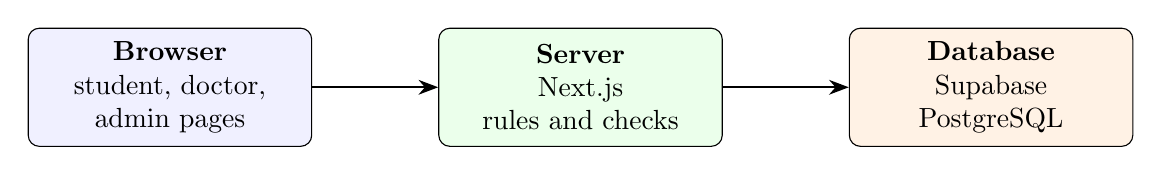
\begin{tikzpicture}[
  box/.style={draw,rounded corners,minimum width=3.6cm,minimum height=1.5cm,align=center,fill=blue!6},
  arr/.style={-{Stealth[length=2.5mm]},thick}]
\node[box] (b) {\textbf{Browser}\\student, doctor,\\admin pages};
\node[box,right=1.6cm of b,fill=green!8] (s) {\textbf{Server}\\Next.js\\rules and checks};
\node[box,right=1.6cm of s,fill=orange!10] (d) {\textbf{Database}\\Supabase\\PostgreSQL};
\draw[arr] (b) -- (s);
\draw[arr] (s) -- (d);
\end{tikzpicture}
\caption{The three main parts of MediQueue}
\label{fig:overview}
\end{figure}

\subsection{Users}
\begin{itemize}
  \item \textbf{Student:} fills in the symptom form, sees the priority score, books a slot and follows the status of the booking.
  \item \textbf{Doctor:} sees the waiting list, updates the status of a visit and writes notes.
  \item \textbf{Admin:} sees schedule information and the audit log. The admin does not see complaints, symptoms or notes.
\end{itemize}

\subsection{Database}
The database has three tables:
\begin{itemize}
  \item \textbf{users:} name, campus ID, email and role.
  \item \textbf{appointments:} the student, complaint, symptoms, severity, score, urgency, slot, status and the encrypted notes.
  \item \textbf{audit\_logs:} time, user, role, action, item and IP address of every important action.
\end{itemize}
A rule in the database stops two active appointments from using the same slot. Another rule stops anyone from changing or deleting audit records.

\subsection{Triage Score}
The priority score is calculated like this:
\[
\text{Score} = (2 \times K) + (1.5 \times S)
\]
\begin{itemize}
  \item $K$ is the \emph{keyword weight}. It is the total of the weights of the symptoms the student ticks, plus the weights of risk words found in the complaint text.
  \item $S$ is the \emph{severity}, a number from 1 to 10 chosen by the student.
\end{itemize}
The score decides the urgency level:
\begin{center}
\begin{tabular}{@{}ll@{}}
\toprule
\textbf{Score} & \textbf{Urgency}\\
\midrule
25 or more & High\\
15 or more, but less than 25 & Medium\\
Less than 15 & Low\\
\bottomrule
\end{tabular}
\end{center}

The symptoms and their weights are: chest pain 10, shortness of breath 8, high fever 6, headache 3, sprain 2 and mild cold 1. Some words in the complaint text, such as ``bleeding'' (7) or ``dizzy'' (3), also add weight.

\paragraph{Example 1.} A student ticks chest pain and shortness of breath, writes both in the complaint, and sets severity 8. Then $K = 10 + 8 + 10 + 8 = 36$ and the score is $(2 \times 36) + (1.5 \times 8) = 84$. The urgency is \textbf{High}.

\paragraph{Example 2.} A student ticks sprain and sets severity 3. The word ``sprain'' is not written in the complaint. Then $K = 2$ and the score is $(2 \times 2) + (1.5 \times 3) = 8.5$. The urgency is \textbf{Low}.

The score is always calculated again on the server. A user cannot send a higher score from the browser to get a better place in the queue.

\subsection{Appointment Status}
Each appointment moves through these steps: Initiated, Triaged, Scheduled, In-Consultation and Completed. A new booking starts as Scheduled. When the doctor finishes, the status becomes Completed and the slot becomes free again.

%% ============================================================ 6
\section{Requirements}

\subsection{Functional Requirements}
\begin{itemize}
  \item The system shall allow users to register and log in with a campus ID and password.
  \item The system shall send each user to the page for their role.
  \item The system shall let a student enter a complaint, choose symptoms and set a severity from 1 to 10.
  \item The system shall show a live priority score while the student fills in the form.
  \item The system shall calculate the final score and urgency on the server.
  \item The system shall let a student book one of the available time slots for today.
  \item The system shall not allow two active appointments in the same slot.
  \item The system shall show students only their own appointments.
  \item The system shall show doctors the waiting list ordered by urgency and then by time.
  \item The system shall let doctors search and filter the list and update the status of a visit.
  \item The system shall let doctors write notes, and shall store the notes in encrypted form.
  \item The system shall show notes only to doctors.
  \item The system shall show administrators the schedule but not complaints, symptoms or notes.
  \item The system shall record important actions in an audit log that cannot be changed.
  \item The system shall let only administrators read the audit log.
\end{itemize}

\subsection{Non-Functional Requirements}
\begin{itemize}
  \item \textbf{Privacy:} private clinical information must be protected from people who do not need it.
  \item \textbf{Security:} access to every server function must be checked by the server, not only by the browser.
  \item \textbf{Reliability:} data must be saved and read correctly, and double booking must not happen.
  \item \textbf{Usability:} each role should have a simple page that is easy to use without training.
  \item \textbf{Maintainability:} the code should be organised so that new features can be added easily.
\end{itemize}

%% ============================================================ 7
\section{Using the System}
This section explains the main screens of the system. All three users log in from the same page.

\subsection{Login and Registration}
A user can sign in with a campus ID and password, or with a Google account. The login page also has quick buttons that fill in the demo accounts. A new user can create an account by entering a name, campus ID, role and password.



\subsection{Student Page}
The student page is used in the following way:
\begin{enumerate}
  \item The student writes the main complaint in the text box.
  \item The student moves the slider to set the severity from 1 to 10.
  \item The student ticks the symptoms that apply.
  \item The page shows the priority score, the urgency level and the calculation at once.
  \item The student chooses a time slot for today. There are 11 slots, from 09:00 to 15:00. The first two slots (09:00 and 09:30) are kept for High urgency.
  \item The student presses \textbf{Confirm Booking}. A message confirms the booking.
  \item Under \textbf{My Appointments}, the student can follow the status of each booking.
\end{enumerate}


\subsection{Doctor Page}
The doctor page is used in the following way:
\begin{enumerate}
  \item The top of the page shows summary cards: total appointments, high priority cases, active and completed visits, and the average severity.
  \item The doctor can search by student ID, name or complaint, and can filter the list by urgency or by active and completed visits.
  \item The doctor selects a patient to see the complaint, symptoms, score and status.
  \item The doctor starts the consultation, writes notes and saves them. The notes are encrypted before they are stored.
  \item The doctor marks the visit as completed after a confirmation message. The slot becomes free.
\end{enumerate}


\subsection{Admin Page}
The admin page shows summary cards and a table with the student ID, slot, status and urgency of each appointment. It also shows the audit log, which lists the time, user, role, action, item and IP address for each important action. Complaints, symptoms and notes are not shown on this page.


%% ============================================================ 8
\section{Results and Analysis}

\subsection{Work Done So Far}
The main parts of the system are working:
\begin{itemize}
  \item Login, registration and separate pages for students, doctors and admins.
  \item The triage score, the live preview on the student page, and the priority-ordered list for doctors.
  \item Slot booking with a check against double booking.
  \item Encrypted consultation notes.
  \item The audit log and the admin view without private details.
  \item On the doctor page: search, filters, summary cards and a confirmation before completing a visit.
  \item On the admin page: summary cards and a layout that works on small screens.
  \item Messages (toasts) that confirm a booking.
\end{itemize}

\subsection{Testing}
Automated tests were written for the most important parts. They run on a computer without a real database.
\begin{itemize}
  \item \textbf{Triage tests} check the urgency limits, the symptom weights, the keyword matching and the allowed severity values.
  \item \textbf{Encryption tests} check that notes can be locked and unlocked correctly, and that damaged or wrongly keyed data is rejected safely.
  \item \textbf{Access tests} check that students see only their own data, that admins do not receive complaints or notes, that only doctors can update consultations, and that only admins can read the audit log. Our QA notes record 22 passing tests for this part.
\end{itemize}
A manual test plan for all three roles has also been written. Running it and recording the results is still to be done.

\subsection{Known Limitations and Planned Fixes}
While reviewing the code, we found some weak points. They are not unusual for a project that is still in progress, and we plan to fix the most important ones in the remaining time.
\begin{enumerate}
  \item \textbf{Choosing a role when registering.} The registration form currently lets a user choose the doctor or admin role. Registration should create students only, and staff accounts should be created another way.
  \item \textbf{Open demo setup link.} The link used to create demo data and to reset it does not ask for a login. It should be limited to administrators or to development use.
  \item \textbf{Priority slots.} The rule that keeps 09:00 and 09:30 for High urgency is checked only in the browser. The server should check it too.
  \item \textbf{Booked slots are not visible to students.} A student sees only their own bookings, so a slot taken by someone else looks free until the booking fails. The page should get a safe list of taken slots.
  \item \textbf{Admin data.} The admin page does not show severity, but the server still sends it. This should be removed or the page note should be corrected.
  \item \textbf{Encryption key.} If no key is set, a built-in test key is used. The system should refuse to start without a proper key.
\end{enumerate}
Other improvements we have noted are a limit on bookings per student, cancelling and changing bookings, a print view of the daily schedule, and a confirmation before the admin resets demo data.

%% ============================================================ 9
\section{Conclusion and Future Work}
MediQueue already shows the main idea of the project: patients are placed in order by urgency, private notes are protected, and every important action is recorded. Students, doctors and admins each have their own page with the information they need.

The project is not finished yet. In the remaining two weeks, the team plans to:
\begin{itemize}
  \item fix the main limitations listed in Section 8.3;
  \item finish the remaining interface tasks, such as the print view and the confirmation before the demo reset;
  \item run the manual test plan and record the results;
  \item add screenshots to this report and update it with the final results;
  \item prepare the presentation slides and the demo.
\end{itemize}
After the course, the system could be extended with cancelling and changing bookings, future-date booking, notifications and a better way to understand the symptoms a student writes.

\end{document}
